\chapter{Implementation} \label{IMPLEMENTATION}

\section{Firebase Configuration} \label{FIREBASECONFIGURATION}
    \subsection{Firestore Structure} \label{DATAIMPLEMENTATION}
    Each of the 4 data classes in this application is represented by a JSON file in the file structure of the Firestore. The 4 data classes are represented in the application by either a Kotlin Data Class \cite{KOTLINDATACLASS}, or a data class like a class with some additional methods for Parcelable functionality. The files are set up in a certain structure for the data to be retrievable using these classes. The idea is that each of the fields in the JSON files is represented by 1 variable in the data classes if the JSON file has a string, then a string with the same name as the JSON variables key is used in the data class. For example, a JSON file that looks like this:
    
\begin{verbatim}
    {
    "name": "MyName"
    "age": "MyAge"
    "location": "Location"
    }
\end{verbatim}
    
    Is accessible as a data object in Kotlin formulated like this:
    
\begin{verbatim}
    data class user(
        var name: String? = "",
        var age: String? = "",
        var location: String? = ""
    )
\end{verbatim}

    Data class examples can be found in the Appendix Section \ref{DATACLASSEXAMPLE}, while only one is strictly a Data Class this is due to the limitations; however, the outwards API of the classes shown the in the Appendix Section \ref{DATACLASSEXAMPLE} are the same when interacting with them as a Data Class.
    
    The Firestore consist of collections, each collection consists of documents, each document can have a field which contains a collection so that the Firestore can hold nested file structures. The top-level collections for this app are:
    
    \begin{itemize}
        \item adoptionProcesses
        \item cats
        \item feedback
        \item users
    \end{itemize}
    
    \subsubsection{AdoptionProcesses Collection}
    The documents in the adoptionProcesses collection are named after the UID of the user that is adopting the cats. Each document then has a collection inside of it called adoptionProcesses. The nested field collection of adoptionProcessed contains documents named the catId of the cat the user wants to adopt, each document in this nested collection contains DocumentReferences (A Firestore data type) that point to the user's document in the user's collection (Section \ref{USERSCOLLECTION}) and the cat's document in the cat's collection (Section \ref{CATSCOLLECTION}), and the status of the current adoption. The status of the adoption is in the form of a key-value pair map object, which contains 5 fields, accepted (Boolean), rejected (Boolean), pending (Boolean), pendingReason (String), and rejectedReason (String). To see what it would look like, look at Figure \ref{fig:adoptionProcessFileStructure} which describes the adoptionProcesses collection using UML Class diagram as a basis for the JSON files.
    
\begin{figure} [htbp!]
    \centering
    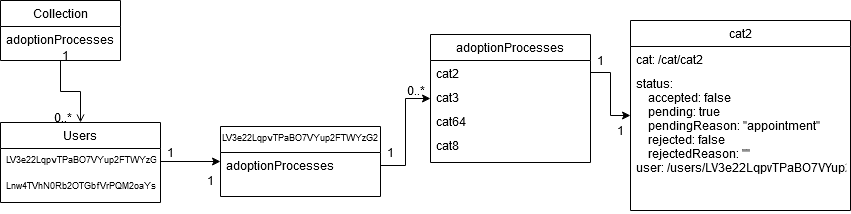
\includegraphics[width=\textwidth]{Images/adoptionProcesses file relations.png}
    \caption{Adoption Processes collection structure}
    \label{fig:adoptionProcessFileStructure}
\end{figure}

    
    \subsubsection{Cats Collection} \label{CATSCOLLECTION}
    The documents in the cat's collection are named after the Cat ID by concatenating the word cat with the id. This is to avoid it just being numbers and being harder to read. The contents of the documents are all of the information the application requires for the cat information displays, and all information is displayed in the app that is stored in these documents. An example of the file structure is given in the form of a UML class diagram representing the JSON files in Figure \ref{fig:catsCollectionFileStructure}
    
\begin{figure} [htbp!]
    \centering
    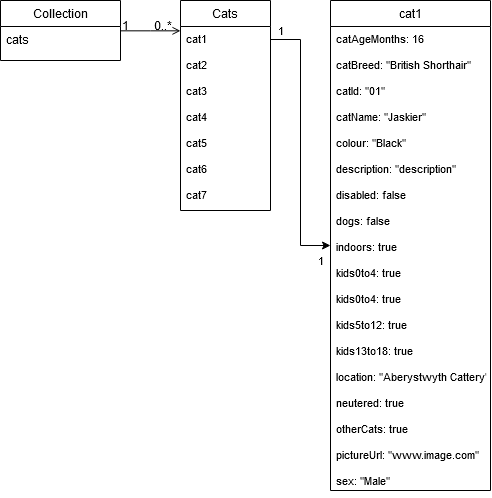
\includegraphics[width=\textwidth]{Images/CatsCollectionFileStructure.png}
    \caption{Cats Collection File Structure}
    \label{fig:catsCollectionFileStructure}
\end{figure}
    
    \subsubsection{Feedback Collection}
    The feedback collection is a collection of the feedback given by users from the app. The feedback documents are small; they contain the date, developerReplyRequested, the feedback, and a reference to the user's document. The feedback document names are a concatenation of their user Ids and the date-time. An example of feedback collection JSON structure is shown in Figure \ref{fig:feedbackCollectionFileStructure} as a UML Class diagram.
    
 \begin{figure} [htbp!]
    \centering
    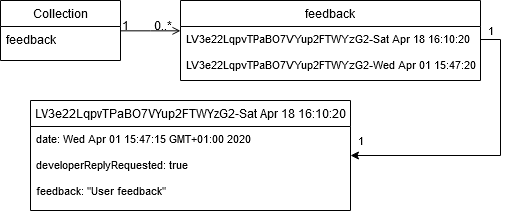
\includegraphics[width=\textwidth]{Images/FeedbackCollectionFileStructure.png}
    \caption{Feedback collection file structure}
    \label{fig:feedbackCollectionFileStructure}
\end{figure}  
    
    \subsubsection{Users Collection} \label{USERSCOLLECTION}
    The user's collection is the collection of user data, and each document has the name of the user's ID; the user ID is gained from the Firebase Authentication implementation (Section \ref{FIREBASEAUTHENTICATION}). The user documents contain the user's address, county, favouritedCats, mobileNumber, name, and postCode. An example of the users collection JSON file structure is found in Figure \ref{fig:usersCollectionFileStructure} as a UML Class diagram.
    
 \begin{figure} [htbp!]
    \centering
    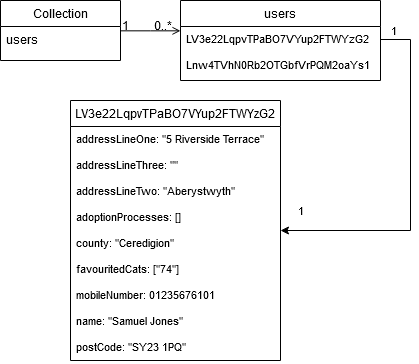
\includegraphics{Images/UserCollectionFileStructure.png}
    \caption{Users collection file structure}
    \label{fig:usersCollectionFileStructure}
\end{figure}   
    
    \subsection{Security Rules}
    The rules have been implemented in a way that restricts access to the database, for everything to some degree. A user must provide an authenticated user id for read or write operations in the user's collection. It is not possible to write to the cat collection, but anyone using a correctly connected application can read cat data. adoptionProcesses data can only be written or read by a correctly authenticated user liked user data. Feedback is unreadable by applications but writable by technically any authenticated application, but the app requires a login.
    
    When a collection is un-readable, or un-writeable by an application connected to the Firestore, this does not include the Firebase console, which allows administrator access to change any values, and read anything.
    
    Security rules for Firebase are easy to update and propagate within 5 minutes across all of the Firebase servers. It provides heavy adaptability at a moments notice so temporary changes could be done if needed like when the Server Scripts are run.
    
    The security rules in use by the Firestore are as follows:
    
\begin{verbatim}
rules_version = '2';
service cloud.firestore {
    match /databases/{database}/documents {
    match /users/{userId} {
        allow read, write: if request.auth.uid == userId
    }
    match /cats/{documents=*}{
        allow read: if true;
        allow write: if false;
    }
    match /adoptionProcesses/{userId}/adoptionProcesses/
                                    {documents=**}{
        allow read, write: if request.auth.uid == userId
    }
    match /feedback/{documents=**}{
        allow write: if true
        allow read: if false
    }
  }
}    
\end{verbatim}

    
    \subsection{Server Scripts} \label{SERVERSCRIPTS}
    The Server Scripts were created when I need to generate a lot of data fast, and I used them with some made-up data in JSON files to create 90 new cat objects. The script for creation was made with the intention to be scale-able, for example, if there was a need for 1 or 1000 extra cats that could be done, the script might get repetitive due to the lack of extra data, but if extra data were added to the JSON files, then it would use it accordingly.
    
    The second script that was made to interact with the server is the remove a certain number of cats script. After the first version of my creates a cat script was created, I realised that 90 cats had been generated incorrectly. The script deletes the cats between 2 numbers input into it in this scenario 10 and 90 was required.
    
    Both scripts required API keys for the Firestore, and these are not available to the public as they are privately linked to my Firestore account. The code in Appendix Sections \ref{CREATECATSCRIPT} and \ref{REMOVECATSSCRIPT}.
    
    Both scripts also use the Cat Class (Appendix Section \ref{CATCLASSSCRIPT}). It makes sense to separate shared code between the scripts, to reduce code duplication, increase stability, and maintainability.

\section{Technologies Used}
This section will talk about how the technologies that have been chosen are implemented in this project. The technologies in question are, Firebase Authentication, Firebase Firestore, Firebase File Storage, Firebase UI Integration Tests, Picasso, Kotlin, Material Design, Android X
    \subsection{Firebase}
    Google Firebase is a set of tools for application developers to integrate into their applications, that are easy to plug in and can quickly implement significant functionality with little effort. While, some features of Firebase make a lot of sense to be implemented on an application going to an audience, since this application is not destined for that path I did not add them, these features include Analytics and Cloud Messaging. This subsection talks about the libraries from Google Firebase that were used and go into detail about their implementation.
        \subsubsection{Authentication and Authentication UI} \label{FIREBASEAUTHENTICATION}
        Firebase Authentication is crucial to the functionality of the application; a large portion of the app is locked behind a login screen. Adoption, Feedback, My Account, and Cat Saving all require correct authentication for all or partial functionality. Authentication can be completed using many 3rd party authentication methods, including Google, Facebook, Twitter, Apple ID and more \cite{FIREBASEAUTHTYPES}. The application only allows for the use of google sign in, which is incredibly easy on Android and most users will have this, and an application-specific email and password. The mentality behind only using the two authentication methods is because it keeps things simple, it reduces chances for users to become confused as to what they signed in with, and it was the two easiest methods to implement.
        
        Firebase Authentication has a support library called Firebase Authentication UI which allows an application to drop in an activity which handles authentication. To do this you "build" the methods that you want to use and pass it to the Activity, when the Activity returns it will return either success or not, with success you are logged in. Firebase Authentication UI is a very nice and easy to use implementation of a login screen, with minimal implementation requirement.
        
        Firebase Authentication UI launch code for Google and Email/password logins:
        \begin{verbatim}
// Choose authentication providers
val providers = arrayListOf(
    AuthUI.IdpConfig.EmailBuilder().build(),
    AuthUI.IdpConfig.GoogleBuilder().build()
)

// Create and launch sign-in intent
startActivityForResult(
    AuthUI.getInstance()
        .createSignInIntentBuilder()
        .setAvailableProviders(providers)
        .setIsSmartLockEnabled(false, true)
        .build(),
    RC_SIGN_IN
)
        \end{verbatim}
        
        It is possible to check the Activity results another way, by calling checking if \newline "FirebaseAuth.getInstance().currentUser" returns a FirebaseUser object, if so there was a successful login for this application, and it has yet to be logged out (This includes if you have just started the application and had previously been logged in), or null if a login has not been performed or the user logged out.

        \subsubsection{Firestore}
        Firebase Firestore is google's latest attempt at providing real-time database support for application development, and it replaced their earlier attempt called Realtime Database, it has simplified security rules and more straightforward implementation on the firebase console. Firestore represents a scalable database implementation in the form of a NoSQL file structure utilising JSON files. Firestore can be interacted with in many ways in multiple languages including, JavaScript, Swift, Objective-C, Java, Java Android, Kotlin Android, Python, C++, Node-JS, GO, PHP, Unity, C\#, and Ruby.
        
        Most of the Firestore configuration and implementation is discussed in section \ref{FIREBASECONFIGURATION}.
        
        \subsubsection{File Storage}
        Google Firebase Storage is a cheap, scalable, secure, and easy to use storage medium in the cloud. In the aspect of this project, it is used to provide storage for cat images. The cat images are easily accessible where anyone can read them from a given URL, these URLs are used in the Firestore (Section \ref{FIREBASECONFIGURATION}) cats collection. 
        
        The security rules are much more basic, this time it is true for all read, and false of all write on all paths in the storage, as it is only storing the cat pictures:
        
        \begin{verbatim}
rules_version = '2';
service firebase.storage {
  match /b/{bucket}/o {
    match /{allPaths=**} {
      allow read: if true;
      allow write: if false;
    }
  }
}
        \end{verbatim}
        
        \subsubsection{UI Integration Tests}
        Google Firebase offers UI Instrumentation tests, which have been used in this project as Integration tests. The project does not make direct use of the Firebase functionality but rather indirectly via Bitrise. The way these tests work is via compiling a test APK using the Android Instrumentation tests and sending it to Firebase to be run on a matrix of testing devices, and the APK can then be run on many types of devices and all Android API levels.
        
        \subsubsection{Firestore Recycler Adapter}
        The FirestoreRecyclerAdapter is used with the RecyclerAdapter, it works using a Firestore query. It will asynchronously populate the RecyclerView and bind the data retrieved by the query to the RecyclerView.ItemHolder. It has been used for all adoption statuses, cat finder tools, and saved cat scrollables. An example of the adapter being setup and given to a RecyclerView is as follows, the adapter needs a FirestoreRecyclerOptions object which first is constructed using the query:
        
\begin{verbatim}
val query = FirebaseFirestore.getInstance()
    .collection("adoptionProcesses")
    .document(DataService.INSTANCE.user!!.uid)
    .collection("adoptionProcesses")
    .limit(10)

val options = FirestoreRecyclerOptions
    .Builder<AdoptionProcess>()
    .setQuery(query, AdoptionProcess::class.java)
    .setLifecycleOwner(this)
    .build()

val adapter =
    object : FirestoreRecyclerAdapter<
    AdoptionProcess, AdoptionStatusCard>(options) {
        override fun onCreateViewHolder
            (parent: ViewGroup, viewType: Int): 
            AdoptionStatusCard {
            val localView = LayoutInflater.from(parent.context)
                .inflate(R.layout.adoption_status_card,
                        parent, 
                        false)
            return AdoptionStatusCard(localView)
        }

        override fun onBindViewHolder(
            holder: AdoptionStatusCard,
            position: Int,
            model: AdoptionProcess
        ) {
            holder.bind(model)
        }
    }
\end{verbatim}

        \subsubsection{Filter Functionality using Queries}
        A key part of the function of the application's cat finder fragment is the implementation of the Firestore query. You can use a Firestore query to filter only specific types of data. This was used to great effect for the cat finder filter functionality, and it boils down to checking if the user wants to filter certain aspects, it is also possible to sort the list in a specific way in reverse orders based on how a user wants. The filter and sort functionality are supported directly by the queries. The cat finder implementation for the query generation is available in Appendix Section \ref{FIRESTOREQUERYIMPLEMENTATION}.
        
        \subsubsection{Adding Packaged APK UID to Firestore}
        In the firebase console, you need to add the SHA Certificate fingerprint, that relates to the bundled APK so that it can send requests to Google Firebase, in order to achieved this, inside Android Studio, you need to run 
        \begin{verbatim}
keytool -exportcert -list -v -alias <your-key-name> /
-keystore <path-to-production-keystore>
        \end{verbatim}
        According to the Firebase Documentation \cite{CLIENTAUTH}, you must add the SHA-1 or SHA256 key that is printed to the terminal to your firebase project settings for the application to interact correctly, this includes the debug, and release versions of the application made on each computer used to compile it unless the key is transferred between each.
        
    \subsection{Picasso}
    Picasso is a Library for Android, to load pictures into an ImageView from a URL, for example over the internet or on the local file system. It is straightforward to use, one line: Picasso.get().load("www.imageUrl.com/image").into(imageView). Picasso asynchronously downloads and inserts the image into the URL, it will cache the images for some time, meaning loading is much faster next time. Every image in the application that is not a Material Design icon is loaded using Picasso. Picasso allows other features such as transformation, use of placeholders, and Debug indicators.
    \subsection{Kotlin}
    Kotlin is a development language that works interchangeably with Java on the Java Virtual Machine. Its main features involve providing concise and easier development in a Java environment. It is the sole language in use for Android development in this project. Kotlin changes the classes and adds subsets such as the Data Classes which are used in this application.
    
    Throughout development, I made heavy usage of the lack of requirement for strong typing for local variables and instance variables that can have their type discerned before compile time. Kotlin boasts heavy co-routine support, and I was unable to utilise this in my project, as most asynchronous parts of the project are handled by 3rd-party libraries, as there is no use to reinvent the wheel.
    
    There are a few features of Kotlin that became very valuable when producing easy and concise code, these are Safe Call and Elvis Call operators. These were used to great effect in the following code excerpt:
\begin{verbatim}
val user = document.toObject<User>()
name.setText(user?.name ?: this.user!!.displayName)
addressLineOne.setText(user?.addressLineOne ?: "")
addressLineTwo.setText(user?.addressLineTwo ?: "")
addressLineThree.setText(user?.addressLineThree ?: "")
postCode.setText(user?.postCode ?: "")
county.setText(user?.county ?: "")
phone.setText(user?.mobileNumber ?: this.user!!.phoneNumber)
\end{verbatim}
    
    \subsection{Material Design}
    While most of Material Design's point, is the guidelines, to assist with the implementation of these guidelines, many of the functionalities suggested have a respective implementation for Android. While some of the guidelines have no implementations, and this application utilises the Material Design implementation of the \gls{Bottom Navigation Bar}, \gls{Card}, \gls{Up Button}, Switches, Text fields, Button, and Navigation Drawer. Material design components are implemented throughout my application, and I believe that they all improve the functionality, look, and general feel of the application.
    \subsection{AndroidX and Jetpack}
        AndroidX is the successor to AndroidCompat as a library, and it aims to support modern features in legacy APIs. Even though features may be in the Android Standard now, that doesn't mean they were previously, and to support these features in earlier APIs we use AndroidX. AndroidX is used so commonly throughout this application that the list would be too long to put in, but some features include ConstraintLayouts, GridLayouts, and the NestedScrollViews.
        
        Android Jetpack is a suite of libraries and tools that are aimed at helping developers write quick and high development applications. Jetpack aims to improve the way developers implement best practices. Android Jetpack is in the namespace of AndroidX; therefore, as a part of AndroidX, Jetpack is discussed as part of the same section.
        \subsubsection{NavigationUI} \label{NAVUI}
        NavigationUI is a relatively new methodology for navigation implementation inside of an Android Application. It utilises a Navigation Graph; the one used in the project is available in Appendix Section \ref{NAVIGATIONGRAPH}. The Navigation graph shows the hierarchy of the application; however since the navigation through this application is relatively simple, it requires only a flat hierarchy of navigation, with HomeFragment being the base of all navigation.
        
        NavigationUI offers the ability to add transition animations, and this application does not currently use them. The reason behind not using them is due to the lack of time, and the idea was to get navigation working before polishing the application later. NavigationUI also handles the animations and up to stack navigation in the app bar between Navigation Draw. NavigationUI is usable throughout the application by calling "findNavController().navigate(fragmentId)".
        
        When you navigate somewhere, it adds this destination to the navigation stack, and when the \gls{Up Button} is pressed then it navigates up the navigation stack to where you previously were in the program.
        
        \subsubsection{Legacy Support for UI Elements} \label{LEGACYUI}
        Grid Layout is a layout that provides an easy to use the grid, and it often is not clear that a grid is used because these items can easily. It's a feature of AndroidX and the current modern Android API, but older versions of the Android SDK do not work with the Grid Layout as it was not implemented, in the case of this application 21-23 did not support Grid Layout, so the AndroidX version was used instead.
        
        Constraint Layout is a performance-friendly easy to use layout for simple and slightly more advanced layouts. It utilises constraints to reduce time spent determining layout sizes dynamically by the CPU, each element or component is placed within relation to another element or the parent using constraints based on their current positions, working from the top of the file downwards, Constraint Layouts are used throughout the project for simple screens that can easily be made as a Constraint Layout, for example, the settings, home, and adoption info view fragment all use the Constraint Layout.

\section{Notable Bugs}
In this section, the notable bugs are discussed as they have significantly impacted development or extra time was needed to source the problem looking at older APIs or discovering the issues, especially with the continuous integration.

    \subsection{Gridlayout - AndroidX}
    As discussed in section \ref{LEGACYUI}, the Grid Layout is not supported in earlier versions of Android. Some functionality used in the My Account screen and user information update screens, are not available in Android 21, 22 or 23. This was evident from the Continuous Integration UI tests, but it was hard to discover precisely what the issue was as it was stating Grid Layout did not inflate as it couldn't be found correctly. The functionality required was the "layout\_columnWeight" and "layout\_rowWeight" which is not supported on these lower APIs.
    
    \subsection{writeBoolean and readBoolean pre API 29}
    Parcelable is an interface implementation that allows a developer to implement it, and it is used quite extensively by the Data Classes in the application (Appendix Section \ref{DATACLASSEXAMPLE}). The data classes required these to be passed between fragments using the NavigationUI navigate methods (Section \ref{NAVUI}). Early on these methods were implemented using a rather new feature writeBoolean and readBoolean, in the UI Integration tests that were running every single device one test ran on, failed except API 29, this was because these two methods had not been implemented until very recently and were not available in a legacy package, so some alternate implementation had to be used.
    
    The alternate implementation was translating a Boolean into a String and back. These are my implementations to facilitate this:

\begin{verbatim}
fun boolToString(bool: Boolean) : String{
    return if (bool) "true" else "false"
}


fun stringToBool(string: String) : Boolean {
    // If not true then assumed false
    return string == "true"
}   
\end{verbatim}
    
    \subsection{Large Image Files Over the Internet}
    
    When the Cat \gls{Card}s were first added to the cat finder tool, it was noticed there was extreme lag, I was concerned this could have been caused by the database being slow or the FirebaseRecyclerAdapter having inefficiencies. However, it ended up being caused by the loading of images; this was because these images were rather large in resolution but being crammed into small ImageViews and processing and download times were causing stuttering and lag. The fix for this was to format and compress the images from their current state without diminishing their quality. I utilised a program called jpegoptim \cite{JPEGOPTIM}, to perform compression, optimisations, and resizing to drop the size of the image from multiple megabytes to below 50 kilobytes, yet still keeping a good enough quality for display on mobile phones.
    
    \subsection{Infinitely Adding to the Navigation Stack in Settings}
    When navigating to the settings screen it was possible to navigate to that screen infinitely from inside of the settings screen, this means that you could in theory infinitely navigate to the settings screen increasing the size of the navigation stack. Whilst not strictly a major problem, it did make it hard to use the \gls{Up Button} to navigate up the navigation stack. The settings navigation button was added to the application's app bar, which means that it is present on every screen, it is possible to remove but required more work to fix correctly than was left in the project. The way this was fixed was by disallowing navigation to the settings destination if already at the settings destination. This code is given in the example:
    
\begin{verbatim}
when (item.itemId) {
    R.id.actionSettingsButton -> {
        if (navController.currentDestination?.id 
                != R.id.settingsFragment){
            navController.navigate(R.id.settingsFragment)
            true
        }
        else
            super.onOptionsItemSelected(item)
    }
    else -> {
        super.onOptionsItemSelected(item)
    }
}
\end{verbatim}
